\documentclass{article}
\usepackage{hyperref}
\usepackage[ngerman]{babel}
\usepackage{amsmath}
\usepackage{amsfonts}
\usepackage{amsthm}
\usepackage{tcolorbox}
\usepackage[a4paper, total={7in, 9in}]{geometry}
\usepackage[font={scriptsize,it}]{caption}
\usepackage{scrextend}
\usepackage{graphicx}
\usepackage{caption}
\usepackage{subcaption}
\usepackage[utf8]{inputenc}
\usepackage[T1]{fontenc}
\DeclareUnicodeCharacter{2212}{-}

% floating figure for column
\newenvironment{Figure}
	{\par\medskip\noindent\minipage{\linewidth}}
	{\endminipage\par\medskip}

\begin{document}

\begin{titlepage}
   \vspace*{\stretch{1.0}}
   \begin{center}
      \Large\textbf{Computertechnik 2 - HS19}\\
      \large\textit{Pascal Brunner - brunnpa7}
   \end{center}
   \vspace*{\stretch{2.0}}
\end{titlepage}


\tableofcontents
\newpage



\section{Microcontroller}
Ein Microcontroller ist eine "Single Chip Solution" mit einem CPU und verschiedenen Peripherie-Geräten (bspw. Timer, Counter, Pulse etc.).
\subsection{Motivation}
Man möchte ein kompaktes System $\rightarrow$ Embedded Systems
\begin{itemize}
	\item tiefe Kosten
	\item Echtzeit
	\item Einsetzbar in extremene Umgebungen (Hitze, Regen, Schnee etc.)
	\item zuverlässig
	\item tiefer Stromverbrauch
	\item tragbar
\end{itemize}
\subsection{Systembus}
Der CPU ist der "Chef" dieses Busses. Der CPU sagt dem Systembus, wann was geschrieben oder gelesen wird. Die Peripheriegeräte und der Speicher agieren nur als "Sklaven", welche Anfrage beantworten. Die Bus-Spezifikation sieht wie folgt aus:
\begin{itemize}
	\item Protokoll und Operationen
	\item Signale $\rightarrow$ Anzahl von Signalen, Signalbeschreibung
	\item Timing $\rightarrow$ Frequenz, Setup and hold times
	\item elektrische Eigenschaften
	\item mechanische Anforderungen
\end{itemize}
Die Signale-Gruppen werden unterteilt in \textbf{Address Linien}:
\begin{itemize}
	\item geht vom Master zum Sklaven 
	\item Anzahl Linien entspricht der Grösse des Adressspeichers
\end{itemize}
\textbf{Daten Linien}:
\begin{itemize}
	\item 8, 16, 32 oder 64 parallele Linien von Daten
	\item bidirektional (read/write)
\end{itemize}
\textbf{Controlsignale}:
\begin{itemize}
	\item Kontrolle read/write Richtung
	\item provide timing information
\end{itemize}

\subsubsection{Bus Timing Option}
Für das Bus Timing gibt es zwei Optionen:\\
\textit{Synchron}\\
\begin{itemize}
\item Master und Sklave verwenden die gleiche Clock
\item Taktflanken (Clock) steuern Bustransfer auf beiden Seiten
\item bei den meisten on-chip Bussen verwendet
\item Off-Chip: DDR und synchroner RAM
\end{itemize}
\begin{Figure}
\centering
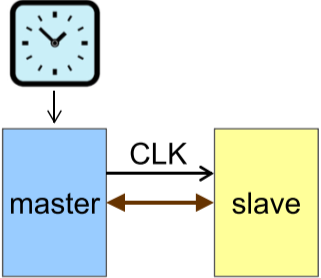
\includegraphics[width=50px]{img/BusTimingSynchron.png}
	\captionof{figure}{Master und Sklave verwenden die gleiche Clock}
	\label{fig:Synchrones Bus Timing}
\end{Figure}

\textit{Asynchron}\\
\begin{itemize}
\item Sklave hat keinen Zugriff auf die Taktflanken (Clock) des Masters
\item Kontrollsignal speichert die Timing-Information um eine Synchronisation zu gewährleisten
\item Vor allem für low data-rate off-chip Speicher gebraucht $\rightarrow$ paralleler Flash-Speicher und asynchroner RAM
\item Off-Chip: DDR und synchroner RAM
\end{itemize}
\begin{Figure}
\centering
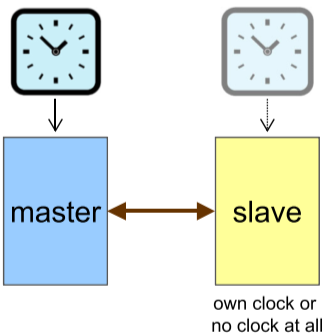
\includegraphics[width=50px]{img/BusTimingAsynchron.png}
	\captionof{figure}{Master und Sklave verwenden unterschiedliche Clocks}
	\label{fig:Asynchrones Bus Timing}
\end{Figure}

\subsubsection{Mehrere Devices verwenden dieselbe Datenlinie}
Mehrere Devices können die gleiche Datenlinien verwenden. Hier kann es zu einem Kurzschluss führen, wenn ein Sklave eine "1" schreibt und der andere Sklave eine "0" schreibt. Denn da wird die das Signal beim Master geerdet.\\
Der CPU definiert welcher Sklave den Datenbus in entsprechender Zeit gebrauchen darf. 
\begin{itemize}
	\item Write		CPU-driver verbindet mit dem Bus		Alle andere Sklaven werden disconnected
	\item Read		CPU-driver nicht verbunden			Nur ein einzelner Sklave ist verbunden, alle andere Sklaven sind nicht verbunden.
\end{itemize}

\subsection{Synchroner Bus}
Internal workings of the system bus are not disclosed by STM. Die Signalnamen, das Bus-Protokoll und die Timing sind basierend auf der externen Synchronität-Modus. Die \textbf{Namenskonvention} bestimmt, dass ein Prefix von "N" (Nxxx) für ein aktives tiefes Signal steht. Des Weiteren steht NOE für \textit{NOT OUTPUT ENABLE}
\begin{itemize}
	\item NOE = 0 $\rightarrow$ output enabled
	\item NOE = 1 $\rightarrow$ output disabled
\end{itemize}
Folgende Signale sind für uns relevant:
\begin{itemize}
	\item CLK
	\item NE = Not enabled $\rightarrow$ Gibt einen Hinweis, dass es ein Start / End von einem Kreislauf ist, active-low
	\item NWE = Not write enabled, active-low
	\item NOE = Not Output Enable
	\item NBL = Not Byte Line $\rightarrow$ Damit erhält man die Möglichkeit Werte in ein WORD zu speichern. 
\end{itemize}

\subsection{Control und Status Register}
\textbf{Control Bits}
\begin{itemize}
	\item erlaubt dem CPU die Sklaven zu konfigurieren
	\item CPU schreibt RegisterBit
	\item Sklaven-Hardware verwendet den Output der RegisterBit
	\item Normalerweise read/write
\end{itemize}
\textbf{Status Bits}
\begin{itemize}
	\item erlaubt dem CPU die Sklaven zu überwachen
	\item Sklave schreibt den Status in das RegisterBit
	\item CPU liest RegisterBit
	\item normalerweise read
\end{itemize}
$\Rightarrow$ Das Gleiche Register kann sowohl die Control, wie auch die Status Bits kontrollieren

\subsection{Address Decoding}
Address Decoding ist die Interpretation der Address-Leitungswerte.\\
\textbf{Full Address Decoding}
\begin{itemize}
	\item Alle Addresslinien sind decodiert (checked)
	\item Ein Control-Register kann genau an einem Ort zugegriffen werden
	\item 1:1 Mapping  $\rightarrow$ Eine eindeutige Addresse zeigt genau zu einem spezifischen Hardware-Register (physikalischer Speicherort)
\end{itemize}

\textbf{Partial Address Decoding}
\begin{itemize}
	\item Nur ein kleiner Teil der Addressen sind decodiert
	\item erkennt einen Address-Bereich oder ein Set von Addressen
	\item n:1 Mapping $\rightarrow$ n eindeutige Addressen zeigen zum gleichen Hardware-Register (physikalischer Speicherort)
	\item Motivation $\rightarrow$ Einfacheres decodieren, Verwendung von Alias
\end{itemize}

\subsection{Langsame Sklaven (Slow Slaves)}
Durch das Einfügen von "Wait-States" kann man die Verwendung von Slow Slaves verbessern. Eine weitere Möglichkeit ist,  dass man eine zusätzliche Kontrollleitung, bei welchem der Sklave sagen kann "ich bin bereit".

\subsubsection{volatile}
Der Compiler kann in gewissen Situation Variablen oder Statements entfernen, wenn es aus Sicht des Compiler nicht benötigt wird. Mit \textit{volatile} stellt man sicher, dass der Zugriff auf die Variabel jeweils auf den effektiven Wert auf der Hardware zugegriffen wird. Und dass der Compiler diesen Wert nicht reduziert oder verändert. Dadurch wird sichergestellt, dass die Variable sich nicht verändert hat z.B. durch andere Prozesse oder Threads. 


\section{Memory}
\begin{Figure}
\centering
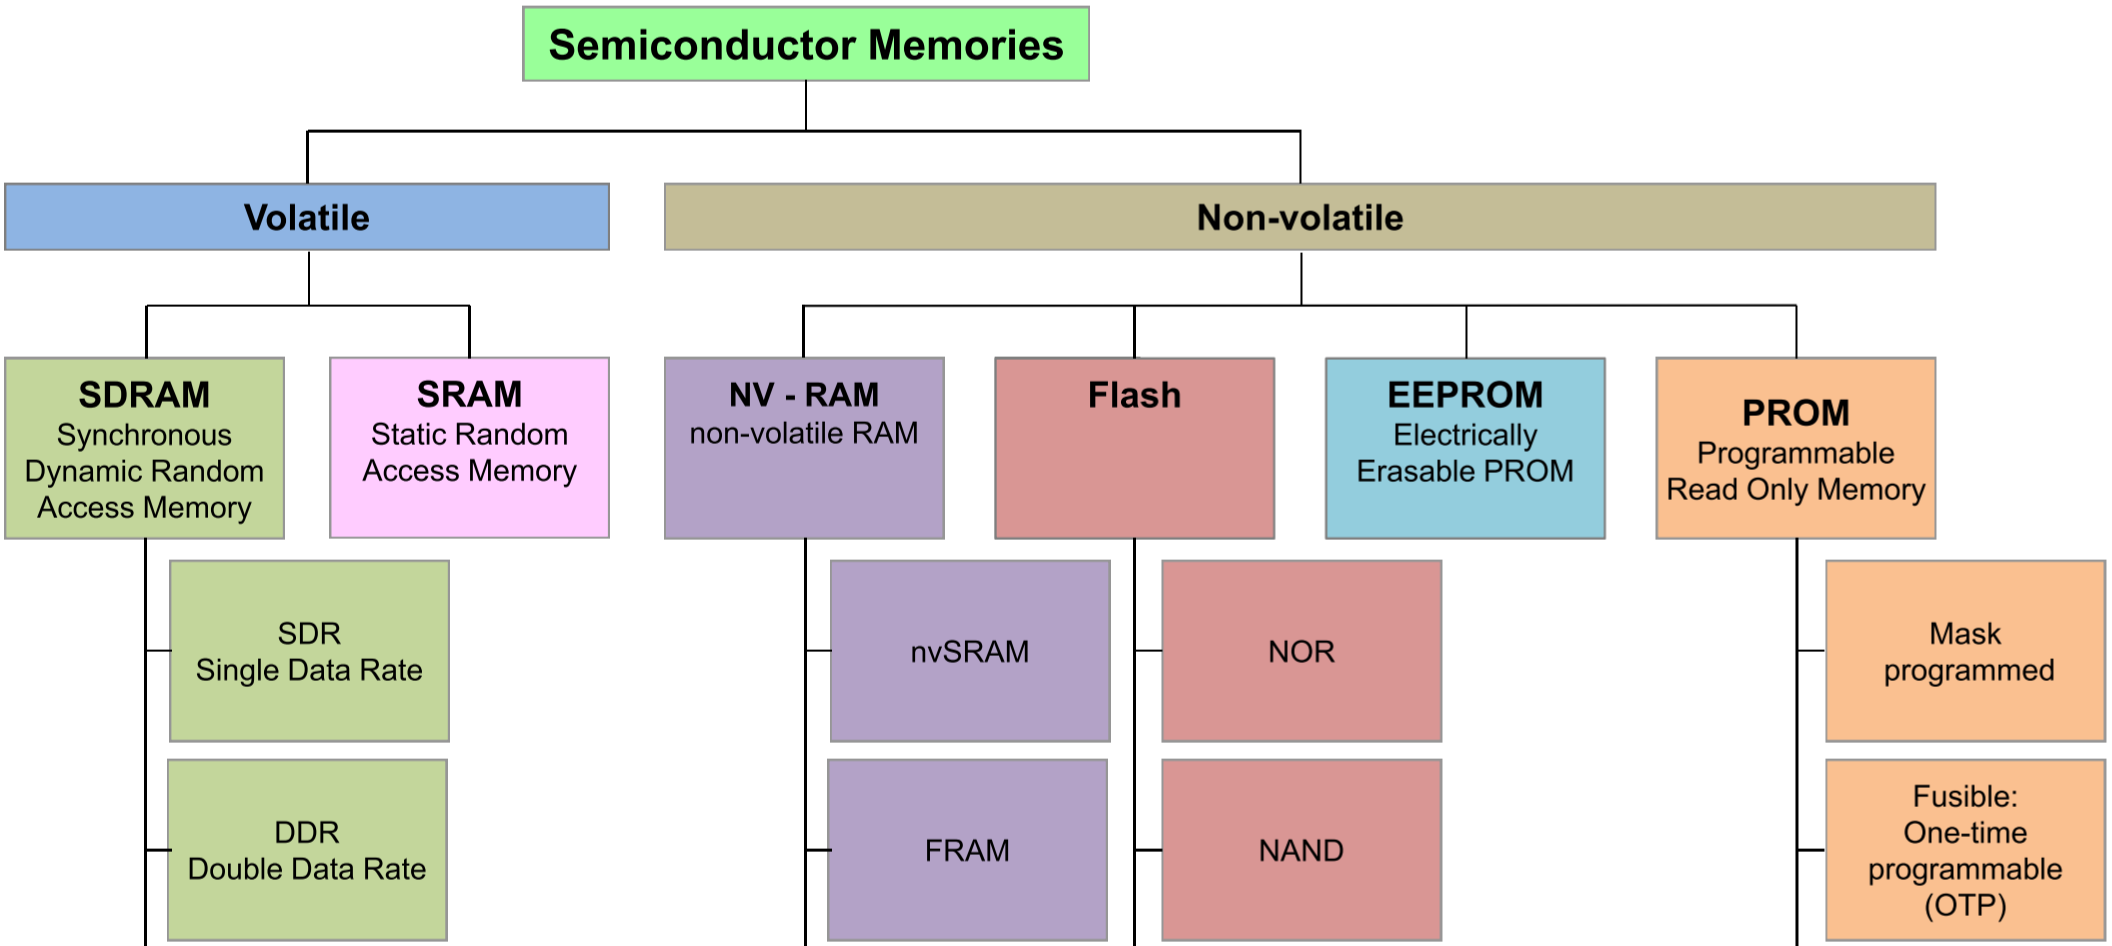
\includegraphics[width=200px]{img/Speicherarten.png}
	\captionof{figure}{Übersicht der einzelnen Speicherarten}
	\label{fig:Übersicht der einzelnen Speicherarten}
\end{Figure}

\subsection{Die unterschiedlichen Einheiten}
\begin{itemize}
	\item{\textbf{Unit Symbols}
	\begin{itemize}
		\item $b = bit$
		\item $B = Byte$
	\end{itemize}	
	}
	\item{\textbf{Memory Chips} $\rightarrow$ Binäre prefixes gemäss JEDEC und IEC
	\begin{itemize}
		\item Kilo \quad K \quad $= 1024$ 
		\item Mega \quad M \quad $= 1024 * 1024$ \quad $=1'048'510$
		\item Giga \quad G \quad $= 1024 * 1024 * 1024$ \quad $=1'073'741'824$
	\end{itemize}
	}
	\item{\textbf{Hard Disks} $\rightarrow$ Often Use SI (or metric) prefixes
	\begin{itemize}
		\item Kilo \quad k \quad $= 1000$ 
		\item Mega \quad M \quad $= 1000 * 1000$
		\item Giga \quad G \quad $= 1000 * 1000 * 1000$
	\end{itemize}
	}
\end{itemize}

\subsection{CT System im Überblick}
\textit{ein vereinfachtes Model des STM32F429ZI}
\begin{itemize}
\item on-chip bus: $\rightarrow$ 32 Datenlinien, 32 Addresslinien und Kontrollsignale
\item external bus: $\rightarrow$ 16 Datenlinien, 26 Addresslinien und Kontrollsignale
\end{itemize}
\begin{Figure}
\centering
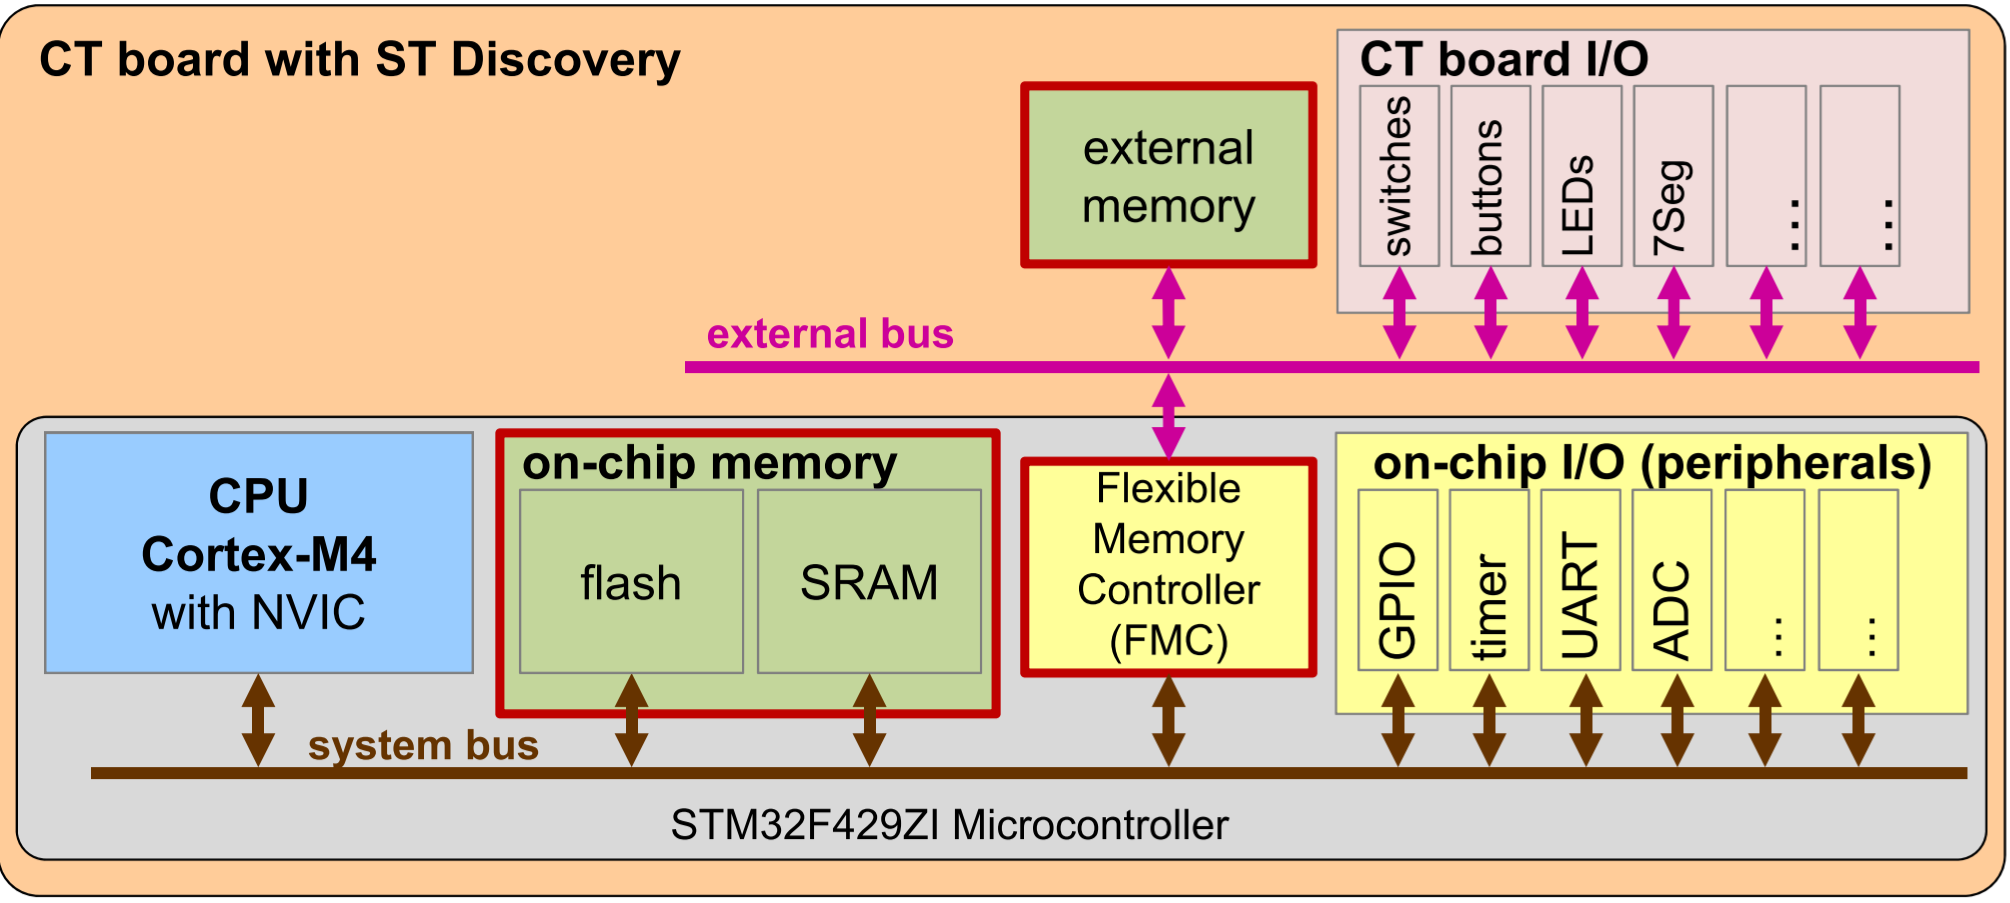
\includegraphics[width=200px]{img/vereinfachtesModellCTBoard.png}
	\captionof{figure}{CT board mit ST Discovery}
	\label{fig:CT board mit ST Discovery}
\end{Figure}

\subsection{On-chip Speicher: SRAM}
SRAM steht für Static Random Access Memory

\begin{itemize}
	\item{Lesen und Schreiben\\
	\begin{itemize}
		\item Alle Zugriffe brauchen ungefähr die gleiche Zeit
		\item Zugriffszeit ist unabhängig wo die Daten im Speicher liegen
		\item Zugriffszeit ist unabhängig vom vorherigen Zugriff
	\end{itemize}
	}
	\item {volatile
	\begin{itemize}
		\item Speicherinhalt ist nur solange verfügbar wie der Speicher angeschalten ist
	\end{itemize}		
	}
	\item {static
	\begin{itemize}
		\item Speicher Elemente sind identisch zu flip-flops
		\item \textbf{Kein} refresh notwendig $\rightarrow$ periodisches Lesen und Umschreiben der Speicherzelle, um den Inhalt zu erhalten.
	\end{itemize}
	}
	\item {Address Regionen
	\begin{itemize}
		\item SRAM1 112K bytes
		\item SRAM2 16K bytes
		\item SRAM3 64K bytes
		\item CCM 64K bytes
	\end{itemize}
	\begin{Figure}
	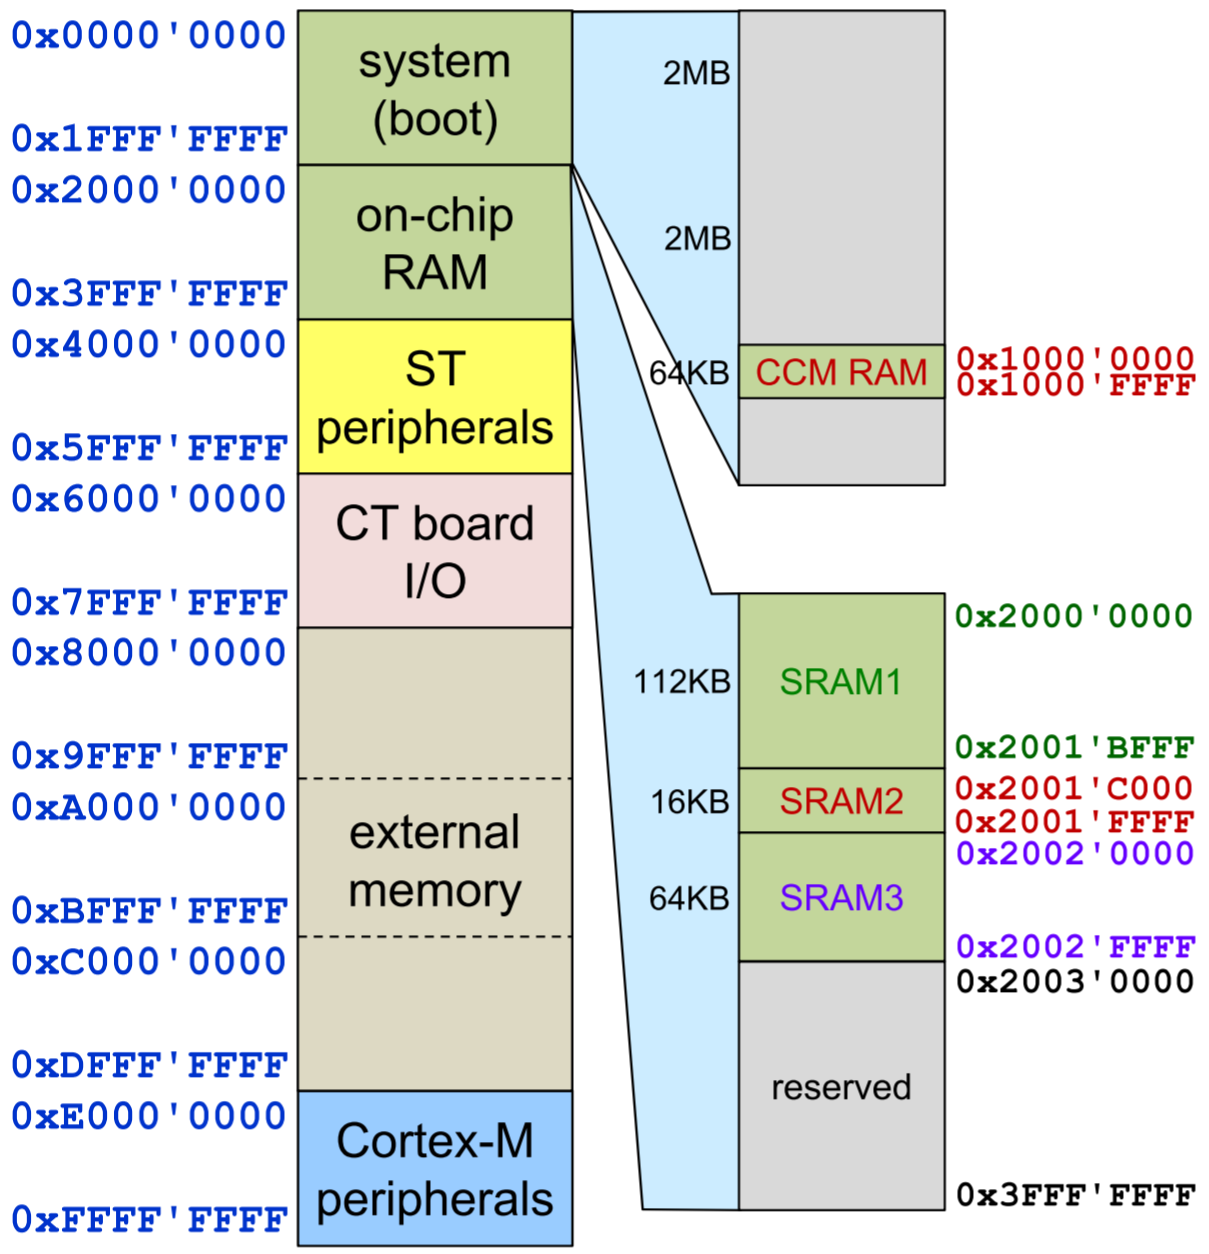
\includegraphics[width=150px]{img/AddressRegionenSRAM.png}
	\captionof{figure}{Die Address Regionen eines SRAM Speichers}
	\label{fig:Die Address Regionen eines SRAM Speichers}
	\end{Figure}		
	}
	\item {Schreiben einer Row (Word):\\
	set bit lines b and !b to (1,0) or (0,1) respectively $\Rightarrow$ Set the addressed word line to 1 $\Rightarrow$ Data is stored in cells $\Rightarrow$ Set word line to 0	
	}
	\item {Lesen einer Row (Word):\\
	pre-charge both bit lines b and !b to 1 $\Rightarrow$ Briefly set word line to 1 $\Rightarrow$ inverts pull either b or !b \underline{towards} (not to ground) $\Rightarrow$ Sense amplifier amplifies small voltage difference between lines b and !b
	\begin{Figure}
	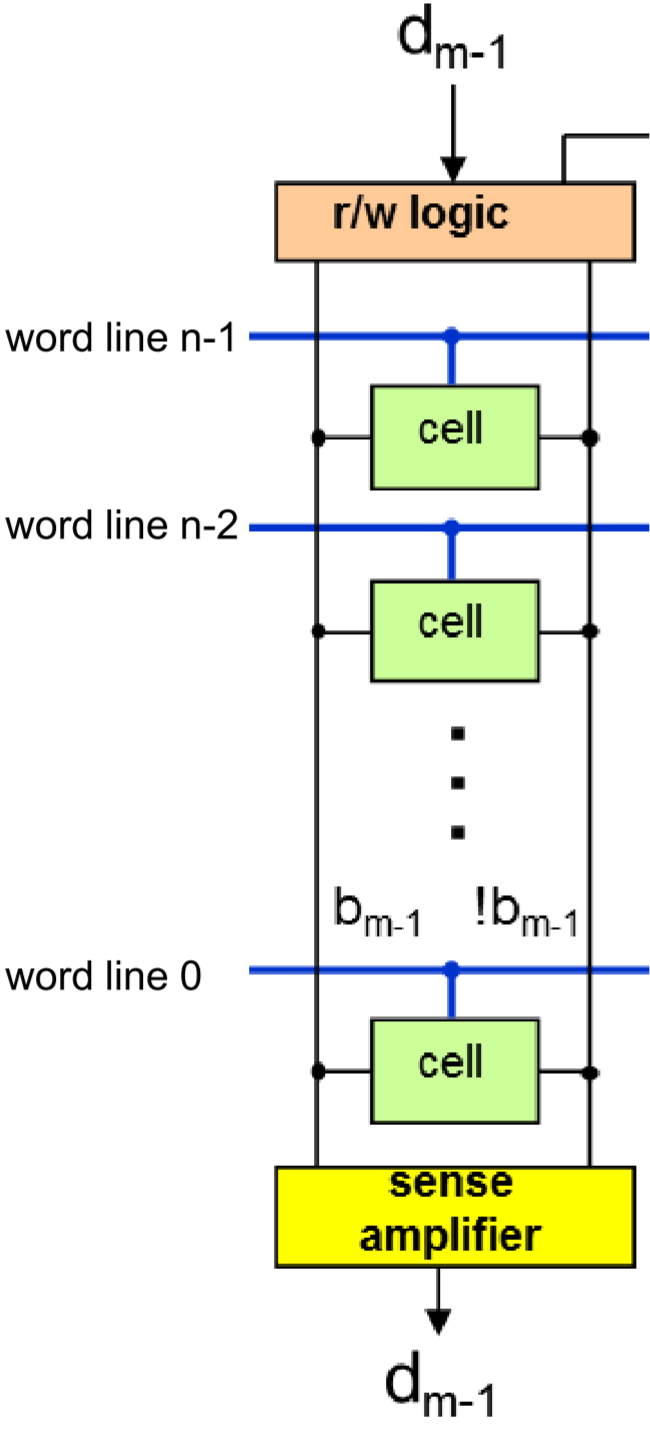
\includegraphics[width=100px]{img/SchemaFuerRWRowSRAM.png}
	\captionof{figure}{Das Schema für das Lesen und Schreiben einer Row (Word) auf einem SRAM}
	\label{fig:Schema RW Word SRAM}
	\end{Figure}		
	}
\end{itemize}

\subsection{Flash}

\section{GPIO}


\end{document}